\section{Theoretischer Hintergrund}
Dadurch bedingt, das diese Arbeit sich an vielen Konzepten aus der Signaltheorie, Elektrotechnik und Informatik bedient, ist es sinnvoll vorab einige Begriffe und Konzepte zu definieren und zu erläutern. Aus diesem Grund, werden im Folgenden das I²C Protokoll, die Grundlagen von Neuronalen Netzen sowie die verwendete Software näher erläutert. 

\subsection{Hybrid-Buck-Wandler}
Bei dem Buck-Wandler handelt es sich um einen DC-DC Wandler, d. h. dieser nimmt eine Gleichstrom Eingangsspannung von 15 bis 40 Volt entgegen und setzt diese herunter auf eine Gleichstrom Ausgangsspannung von 12 Volt. Des Weiteren ist der hier verwendete Wandler auf einen Stromfluss von 10 Ampere limitiert, was bedeutet, dass die maximale Leistung am Ausgang des Wandlers 120 Watt beträgt. Es bedeutet ebenfalls, dass, wenn der Strom 10 A übersteigt, die Ausgangsspannung gedrosselt wird.
Der Wandler besitzt ebenfalls eine I²C Schnittstelle, aus welcher Ausgangsspannung, Eingangsspannung, Ausgangsstrom und Temperatur des Boards gemessen und ausgelesen werden können. Die Datenleitungen des I²C Busses sind bereits auf dem Wandler selbst mit Pull-Up Widerständen ausgestattet, wodurch diese nicht in externen Schaltungen realisiert werden müssen. 

\subsection{I2C}
I2C steht für Inter-Integrated Circuit und wurde von Philips Semiconductors 1982 entwickelt. Es handelt sich dabei um einen seriellen Datenbus im Master-Slave Stil. Dieses Protokoll setzt auf zwei Leitungen für den Datenaustausch, davon ist ein Kanal explizit für die Daten vorgesehen und der andere Kanal für den Takt. Der Takt beträgt im klassischen 100 KHz oder 400 KHz. 

\begin{figure}
    \centering
    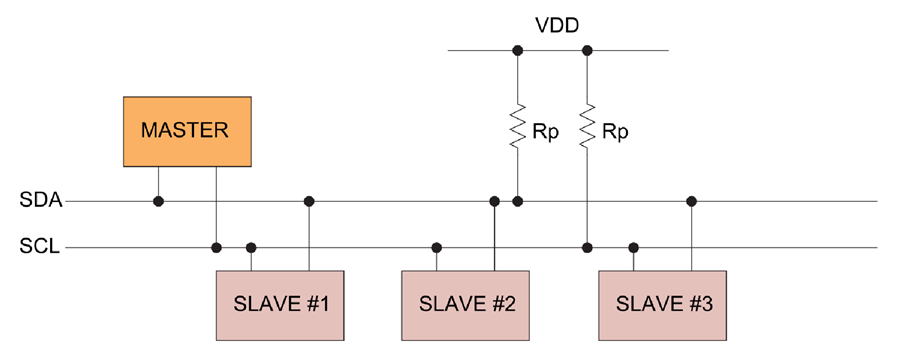
\includegraphics[height= 5cm, width = 10cm]{Pictures/I2C_Bus.png}
    \caption{I2C Bus Beispiel Quelle: https://www.analog.com/en/technical-articles/i2c-primer-what-is-i2c-part-1.html}
\end{figure}

Es ist zu erkennen, dass es eine Master- und mehrere Slave Komponenten gibt. Der Master gibt allen Slaves vor, was sie zu senden haben, und wie schnell sie es tun sollen. Des Weiteren ist zu erkennen, das die beiden Leitungen SDA und SCL an einem Pull-Up Widerstand angeschlossen sind. Dieser dient dazu, die Leitungen, wenn weder Master noch Slave sendet, auf die Versorgungsspannung zu schalten, sodass keine undefinierten Zustände entstehen und die Leitung im unbenutzten Zustand eine logische 1 besitzt. Die Kommunikation erfolgt durch Adressen, so besitzt jeder Sensor eine I2C Slave Adresse, über die ein Master auf diese zugreifen kann. Das auslesen der Daten eines Slaves erfolgt per Registeradressen, so hat beispielsweise ein beliebiger I²C fähiger Sensor ein Register, in dem bestimmte Werte gespeichert sind. In dieser Arbeit handelt es sich bei dem I2C Slave um einen Mikrocontroller auf dem Buck-Wandler. Der Master ist dabei ein Raspberry Pi, welcher direkt per I2C mit dem Netzteil verbunden werden kann.
\end{flushleft}



\subsection{Neuronale Netze}

Zur durchführung einiger simpler Testfälle unter den Punkten 3.2.1 und 3.2.2 ist es notwendig, eines der Grundlegenden Konzepte von Machine Learning zu erläutern: das Neuronale Netz.
Neuronale Netze gehören zur Maschine Learning Kategorie des "supervised learning". Beim supervised learning wird ein neuronales Netz anhand von Eingabedaten (Input) und bereits definierten Lösungen (Output) daraufhin optimiert, bei gegebenen Input eine passende Lösungsstrategie für den bereits definierten Output zu finden. 


\begin{figure}
    \centering
    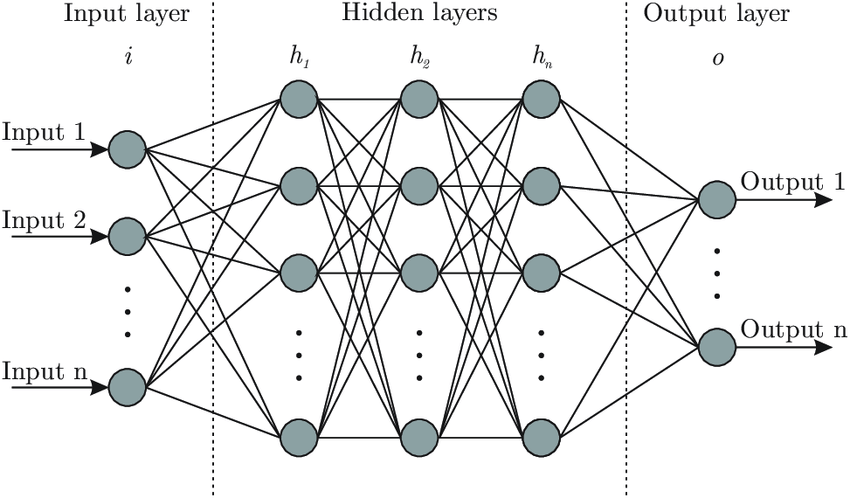
\includegraphics[height= 5cm, width = 10cm]{Pictures/NN_Concept.png}
    \caption{Beispiel eines Neuronalen Netzes: https://www.researchgate.net/figure/Artificial-neural-network-architecture-ANN-i-h-1-h-2-h-n-o_fig1_321259051}
\end{figure}


In Abb. 2 erkennt man eine Abbildung der Architektur eines möglichen neuronalen Netzes. Dieses ist aufgeteilt in mehrere Schichten: Input layer,hidden layer, Output layer. Das Input layer nimmt die Daten auf, welche verarbeitet werden müssen. Diese Daten können von verschiedener Art sein, so können es z. B. Pixeldaten eins Bildes sein, oder der Zeitverlauf von einem Signal. Im hidden layer werden die Daten durch diverse mathematische Operationen verarbeitet, um im Output layer Aussagen über die Input Daten machen zu können, d. h. um die Input Daten zu klassifizieren. Neben den einzelnen Schichten ist zu erkennen, dass es mehrere Knoten gibt, welche untereinander durch Kanten vollvermascht sind. Die Knoten werden im Allgemeinen "Neuronen" genannt und die Kanten sind die sog. "weights" oder Gewichtungen. Die Gewichtungen sind dabei die Hauptparameter eines Neuronalen Netzes. Bei Neuronalen Netzen wird zwischen zwei Algorithmen unterschieden, dem Feedforward Algorithmus, welcher bei gegebenen Input Daten und Gewichtungen einen bestimmten Output liefert. Und dem Backpropagation Algorithmus, welcher bei gegebenem Input und Output neue Gewichtungen für das Neuronale Netz berechnet. Im Folgenden werden beide Algorithmen näher erläutert. 



\begin{figure}
    \centering
    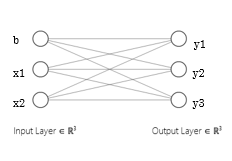
\includegraphics[height= 5cm, width = 6cm]{Pictures/FF.png}
    \caption{Konzept des Feedforward Algorithmus }
    
    


    
          A\Bigg(
         \begin{bmatrix}
           w_{10}  w_{11} \\     
           w_{20}  w_{21} \\           
           w_{30} w_{31}
          \end{bmatrix}
          \begin{bmatrix}
           x_{1} \\
           x_{2} \\
         \end{bmatrix}
         + 
         \begin{bmatrix}
           b_{1} \\
           b_{2} \\
           b_{3} \\
         \end{bmatrix}
            \Bigg)
          =
          \begin{bmatrix}
           y_{1} \\
           y_{2} \\
     
           y_{3}
         \end{bmatrix}
         
 	
          }

\end{figure}
Abb. 3 zeigt ein vereinfachtes Neuronales Netzt mit zwei Schichten. Das Input layer nimmt zwei Eingangswerte entgegen und verrechnet diese per Matrixmultiplikation mit den Gewichtungen, wie in \hl{Gleichung X dargestellt}. Nach dieser Matrixmultiplikation entsteht ein neuer Vektor mit der gleichen Dimension wie der Output layer. Zu diesem Vektor wird noch der sog. "Bias" addiert. Der Bias dient als feste Skalierung dazu, ein Neuron gezielt mehr, bzw. weniger Aktiv zu machen, das bedeutet mathematisch, dass der numerische Wert gezielt gesteigert bzw. verringert wird. Nachdem der Input mit den Gewichtungen und dem Bias verrechnet wurde, wird auf das Ergebnis eine Aktivierungsfunktion angewendet. Eine Aktivierungsfunktion dient dazu zu bestimmen, wie "aktiv" ein Neuron ist. Es existieren mehrere Aktivierungsfunktionen. So zeigen Abbildungen 4 und 5 zwei Mögliche Funktionen. 

Die Formel für die Sigmoid Funktion: 

\begin{equation}
\label{Sigmoid}
s(z) = \frac{1}{1+e^{-z}}
\end{equation}

\begin{figure}
    \centering
    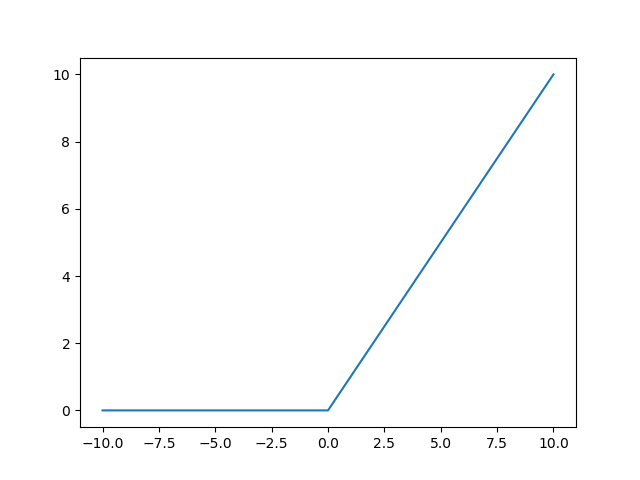
\includegraphics[height= 5cm, width = 10cm]{Pictures/Relu.png}
    \caption{Rectified Linear Unit}
\end{figure}


\begin{figure}
    \centering
    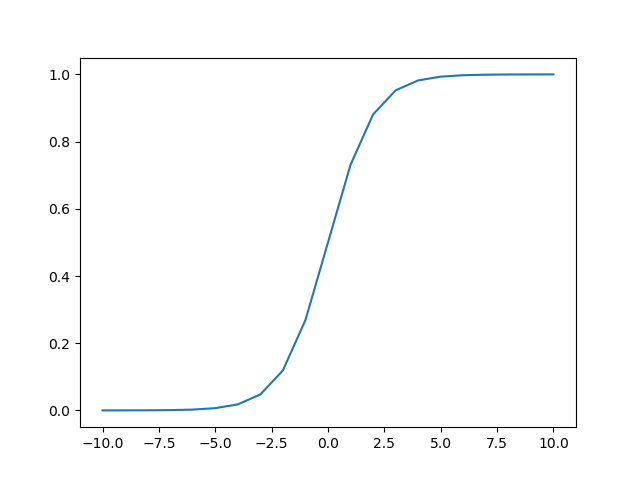
\includegraphics[height= 5cm, width = 10cm]{Pictures/Sigmoid.png}
    \caption{Sigmoid Funktion}
\end{figure}


In Abb. 4 ist eine der \hl{beliebtesten} Aktivierungsfunktionen zu sehen, die ReLu Funktion. Wenn der Input der Funktion <= 0 ist, dann ist der Output immer 0. Für Werte > 0, ist der Output immer der selbe Wert 


\[ y = \left\{ \begin{array}{ll}
         0 & \mbox{if $x <= 0$}\\
	        x & \mbox{if $x > 0$}\end{array} \right. \] 
	        
	        
	        
	        
\subsection{Verwendeten Platformen, Programmiersprachen und Bibliotheken}

Da sich herausgestellt hat, dass ein PicKit eine zu geringe Abtastrate ermöglicht, wurde für die dynamischen Tests ein Raspberry Pi 4 (4 GB RAM) mit der Programmiersprache Python für Datenerfassung- und Verarbeitung verwendet. Des Weiteren wurde für das Erstellen von Neuronalen Netzen die library "Tensorflow" verwendet, wobei Keras als High-Level API dient. Die graphische Visualisierung der Daten erfolgt ausschließlich per Pyplot library.

\end{flushleft}